\documentclass[spanish,12pt,letterpapper]{article}
\usepackage{babel}
\usepackage[utf8]{inputenc}
\usepackage{graphicx}
\usepackage{hyperref}
\usepackage{makeidx}
\makeindex
\begin{document}
	\begin{titlepage}
		\begin{center}
			
\includegraphics[width=0.6\textwidth]{../logoUnADM}~\\[1cm] 
			\textsc{Universidad Abierta y a Distancia de México}\\[0.8cm]
			\textsc{Desarrollo de Software}\\[1.8cm]
			
			\textbf{ \Large Evidencia de aprendizaje. Manual de diagramas del modelado de negocios }\\[3cm]
			
			Diego Antonio Plascencia Lara\\ ES1421004131 \\[0.4cm]
			Facilitador(a): Julia Alicia Reyes Rios\\
			Materia: Modelado de Negocios\\
			Grupo: DS-DMDN-1601-B1-007 \\
			Unidad: IV \\
			
			\vfill México D.F\\{\today}
			
		\end{center}
	\end{titlepage}
	
	\printindex
	
	
	\section{Caso de estudio}
	\index{Caso de Estudio}
	Para esta evidencia utilizare el caso dado ``Aplicaciones de la realidad virtual en la ingeniería'', en el cual retomo ``Las fases del diseño conceptual de ingeniería'', las cuales son:
	\begin{itemize}
	\item Reconocimiento de la necesidad
	\item Definición del problema
	\item Síntesis
	\item Análisis y optimización
	\item Evaluación
	\item Presentación
	\item Visualización
	\end{itemize}
	
	\section{Diagrama de Actividades\\}
	\index{Diagrama de Actividades}
	\begin{center}
	\includegraphics[width=1\textwidth]{./act}~\\[1cm]
	\end{center}
	Este diagrama es simple, pues muestra principalmente las actividades que se llevan a cabo con sus respectivos condicionales si es necesario iterar, asi como sus gateways de paralelismo de tareas. En este diagrama no solo se presentan actividades, sin mencionar actores.
	
	\section{Diagrama Flujo de Funciones Cruzadas\\}
	\index{Diagrama de Flujo de Funciones Cruzadas}
	\begin{center}
	\includegraphics[width=1\textwidth]{./cross}~\\[1cm]
	\end{center}
	Este diagrama es similar al anterior, pero se muestran los actores, y los condicionales están mas detallados.
	
	\section{Diagrama BPMN\\}
	\index{Diagrama BPMN}
	\begin{center}
	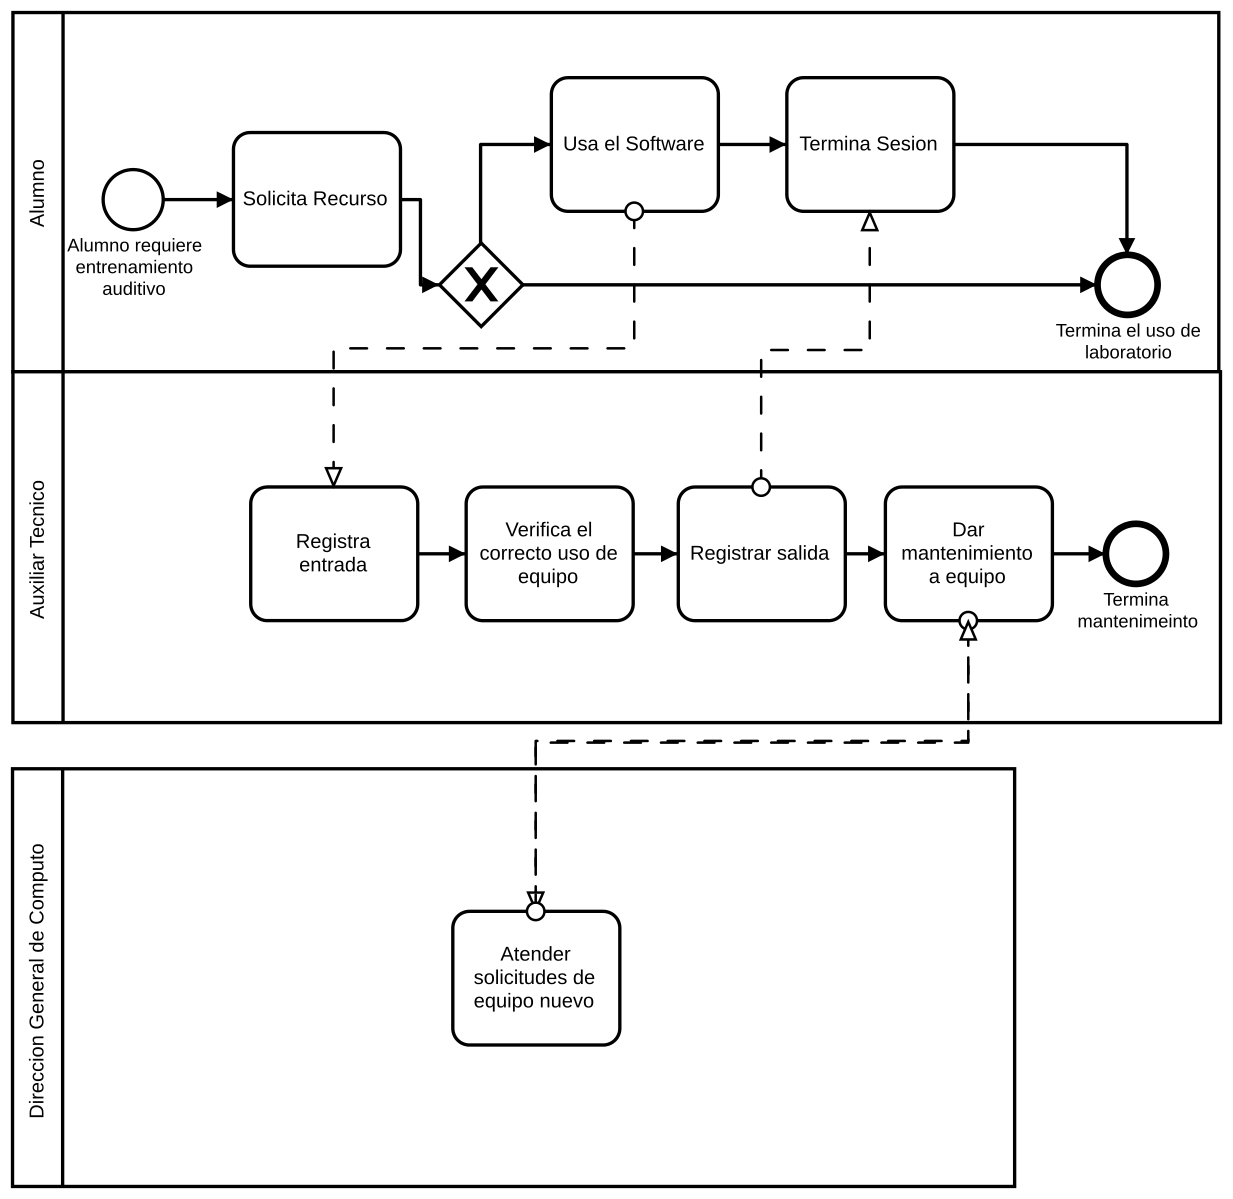
\includegraphics[width=1\textwidth]{./bpmn}~\\[1cm]
	\end{center}
	Este diagrama es similar a los dos anteriores, pues muestra los actores, condicionales, pero en este se usan los artefactos y objetos respectivos de la notación BPMN, así como también se agregan los productos que hay en ciertas actividades, como los requerimientos y el producto, también se muestra donde inicia y termina el proceso.
	
	\section{Diagrama Casos de Uso\\}
	\index{Diagrama Casos de Uso}
	\begin{center}
	\includegraphics[width=1\textwidth]{./usecases}~\\[1cm]
	\end{center}
	En este diagrama se muestran las actividades, y los actores que intervienen en ella, así como las subactividades. Este diagrama es útil para poder ver un poco de los roles y actividades que debe llevar a cabo cada actor.
	
	\section{Modelo Conceptual\\}
	
	\subsection{Diagrama interacción}
	\index{Diagrama de Interacción}
	\begin{center}
	\includegraphics[width=0.7\textwidth]{./interact}~\\[1cm]
	\end{center}
	En este diagrama se pueden observar los objetos y mensajes entre estos, el diagrama es util para tener una noción de donde se concentran los tiempos, asi como de la comunicación entre objetos.
	\subsection{Diagrama comunicación}
	\index{Diagrama de Comunicación}
	\begin{center}
	\includegraphics[width=0.7\textwidth]{./comunic}~\\[1cm]
	\end{center}
	Este diagrama es similar al anterior, pero mas "plano", en el se observa mas el flujo de los mensajes.
	\subsection{Diagrama transición de estados}
	\index{Diagrama de Transición de Estados}
	\begin{center}
	\includegraphics[width=0.3\textwidth]{./states}~\\[1cm]
	\end{center}
	Por ultimo, en este se observa el estado de el proyecto, es útil para saber el ciclo de vida de el proyecto y en que estado se encuentra al pasar por ciertas actividades o en ciertos mensajes entre actores.
	
	\section{Conclusiones}
	En evidencia se retomaron las 4 unidades y se reforzaron todos los diagramas vistos (UML y BPMN). Es importante conocer estos diagramas ya que nos permiten comunicarnos fácilmente por medio de algo visual, por lo que incluso el cliente podría estar informado con poder ver un diagrama sin necesidad de tener conocimientos profundos en ellos, pues son entendibles y fáciles de interpretar.\\
	
	Los diagramas también nos ayudan a tener documentados los procesos, esto sirve en un negocio para hacer análisis y optimización, mejorando así la calidad de servicios o productos ofrecidos, reducir costos y errores, estandarizando así el que hacer de un negocio. 
	

	\pagebreak
	\begin{thebibliography}{9}
	\bibitem{Alexander, Ian. Beus-Dukic, Ljerka} . 
		\emph{Discovering Requirements: How to Specify Products snd Services}. England. Wiley
	
	\bibitem{maturanaModelamiento} Object Management Group. 
		\emph{Business Process Model and Notation}. {[} Fecha de consulta: \today {]}. Disponible en: \textless http://www.bpmn.org/ \textgreater	
	
		\bibitem{maturanaModelamiento} Maturana Ortiz, Jorge. 
		\emph{Modelamiento de Software y Negocios}. {[} Fecha de consulta: \today {]}. Disponible en: \textless http://www.info.univ-angers.fr/pub/maturana/files/Modelamiento\_de\_Software\_y\_Negocios.pdf \textgreater
		
		\bibitem{panAdm} León León, Oyuky María \& Asato España, Julio Armando. 
		\emph{La Importancia del Modelado de Procesos de
			Negocio como Herramienta para la Mejora e
			Innovación}. Panorama administrativo {[}en linea{]}, México. 2009, vol.4 num. 7  {[} Fecha de consulta: \today {]}. Disponible en: \textless http://132.248.9.34/hevila/Panoramaadministrativo/2009/no7/4.pdf \textgreater
	\end{thebibliography}
\end{document}